\documentclass[11pt,a4paper]{article}
\usepackage[utf8]{inputenc}
\usepackage[spanish,es-nodecimaldot]{babel}
\usepackage[margin=2.0cm,top=2.8cm,bottom=2.2cm,headheight=112pt]{geometry}
\usepackage{graphicx}
\usepackage{tabularx}
\usepackage{mathptmx}
\usepackage{fancyhdr}
\usepackage[table,xcdraw]{xcolor}
\usepackage{titlesec}
\usepackage{setspace}
\usepackage{microtype}
\usepackage{lastpage}
\usepackage{booktabs}
\usepackage{enumitem}
\usepackage{amsmath}
\usepackage{amssymb}
\usepackage{multirow}
\usepackage{listings}

\definecolor{codegreen}{rgb}{0,0.6,0}
\definecolor{codegray}{rgb}{0.5,0.5,0.5}
\definecolor{codepurple}{rgb}{0.58,0,0.82}
\definecolor{backcolour}{rgb}{0.96,0.96,0.96}

\lstdefinestyle{mystyle}{
    backgroundcolor=\color{backcolour},   
    commentstyle=\color{codegreen},
    keywordstyle=\color{magenta},
    numberstyle=\tiny\color{codegray},
    stringstyle=\color{codepurple},
    basicstyle=\ttfamily\footnotesize,
    breakatwhitespace=false,         
    breaklines=true,                 
    captionpos=b,                    
    keepspaces=true,                 
    numbers=left,                    
    numbersep=5pt,                  
    showspaces=false,                
    showstringspaces=false,
    showtabs=false,                  
    tabsize=2
}
\lstset{style=mystyle}

\setstretch{1.15}

\titleformat{\section}
  {\fontsize{13}{15}\bfseries\color{headerred}}{\thesection.}{0.5em}{}
  [{\color{headerred}\titlerule[0.8pt]}]

\titleformat{\subsection}
  {\fontsize{11}{13}\bfseries\color{darkred}}{\thesubsection.}{0.5em}{}

\titleformat{\subsubsection}
  {\fontsize{10}{12}\bfseries}{\thesubsubsection.}{0.5em}{}

\titlespacing*{\section}
  {0pt}{1.8ex plus 0.4ex minus 0.2ex}{0.8ex plus 0.2ex}
\titlespacing*{\subsection}
  {0pt}{1.4ex plus 0.3ex minus 0.2ex}{0.5ex plus 0.1ex}
\titlespacing*{\subsubsection}
  {0pt}{1.1ex plus 0.2ex minus 0.1ex}{0.3ex plus 0.1ex}

\newcolumntype{Y}{>{\centering\arraybackslash}X}
\newcolumntype{L}{>{\raggedright\arraybackslash}X}
\newcolumntype{C}{>{\centering\arraybackslash}X}

\definecolor{headerred}{RGB}{180, 0, 0}
\definecolor{darkred}{RGB}{140, 0, 0}
\definecolor{lightgraybg}{RGB}{248, 248, 248}
\definecolor{tableheader}{RGB}{232, 238, 246}

\newcommand{\docCodigo}{TI-SIGE-ENT-S2-002}
\newcommand{\docVersion}{1.0}
\newcommand{\docProceso}{DISEÑO DE SOFTWARE / ARQUITECTURA}
\newcommand{\docElaboracion}{28/08/2026}
\newcommand{\docRevision}{PENDIENTE DE REVISIÓN}
\newcommand{\docTitulo}{DISEÑO DE ARQUITECTURA MODULAR, MODELO C4 Y STACK NODE.JS / POSTGRESQL}
\newcommand{\docOrganizacion}{FACULTAD DE INGENIERÍA EN SISTEMAS, ELECTRÓNICA E INDUSTRIAL}
\newcommand{\docSubOrganizacion}{CARRERA DE INGENIERÍA DE SOFTWARE}

\newcommand{\encabezadofrecuente}{%
    \renewcommand{\arraystretch}{1.15}%
    \noindent\makebox[\textwidth][c]{%
    \begin{tabularx}{\textwidth}{|>{\centering\arraybackslash}m{2.8cm}|Y|>{\centering\arraybackslash}m{4.8cm}|}
        \hline
        \multirow{4}{2.8cm}{\centering\raisebox{-1.15cm}{
\includegraphics[width=2.5cm,height=2.0cm,keepaspectratio]{images/logo.png}}}
        & \textbf{\fontsize{9}{11}\selectfont \docOrganizacion} 
        & \textbf{\fontsize{8}{10}\selectfont CÓDIGO:} \fontsize{8}{10}\selectfont \docCodigo \\
        \cline{3-3}
        & \textbf{\fontsize{8.5}{10.5}\selectfont \docSubOrganizacion} 
        & \textbf{\fontsize{8}{10}\selectfont VERSIÓN:} \fontsize{8}{10}\selectfont \docVersion \\
        \cline{2-3}
        & \textbf{\fontsize{8}{10}\selectfont PROCESO:} \fontsize{8}{10}\selectfont \docProceso 
        & \textbf{\fontsize{8}{10}\selectfont ELABORACIÓN:} \fontsize{8}{10}\selectfont \docElaboracion \\
        \cline{2-3}
        & \textbf{\fontsize{8.5}{10.5}\selectfont \docTitulo} 
        & \textbf{\fontsize{8}{10}\selectfont ÚLTIMA REVISIÓN:} \fontsize{8}{10}\selectfont \textbf{\textcolor{darkred}{\docRevision}} \\
        \hline
    \end{tabularx}%
    }%
}

\pagestyle{fancy}
\fancyhf{}
\fancyhead[C]{\encabezadofrecuente}
\fancyfoot[C]{\fontsize{10}{12}\selectfont Página \thepage\ de \pageref{LastPage}}
\renewcommand{\headrulewidth}{0pt}

\begin{document}

\section{Título}
\textbf{Denominación del Entregable:} Documento de Arquitectura de Software (SAD), Modelo C4 y Patrones de Diseño Modular (EDT 2.2)



\section{Introducción}
La arquitectura de software del sistema \textbf{SIGE} se concibe bajo principios de alta cohesión, bajo acoplamiento, escalabilidad, máxima velocidad de respuesta e independencia modular. Se implementa una \textbf{Arquitectura Modular en Capas basada en Node.js + Express (v5)} y \textbf{PostgreSQL (18)} en el backend, articulada con una interfaz \textbf{Single Page Application (SPA) en React + Vite} potenciada por \textbf{Tailwind CSS}, animaciones fluidas por GPU mediante CSS Keyframes y paleta institucional \texttt{\#00345E} (Azul UTA/FISEI). Esta base técnica se complementa con el \textbf{Modelo C4} para la visualización estructural del sistema y especificaciones rigurosas de seguridad basadas en \textbf{Bcrypt.js}, \textbf{JSON Web Tokens (JWT)} y cabeceras de protección HTTP con \textbf{Helmet}.

\section{Objetivo}

\subsection{Objetivo General}
Diseñar y formalizar la arquitectura modular de software del sistema SIGE mediante Node.js + Express (v5), PostgreSQL 18, React + Vite y el Modelo C4, asegurando mantenibilidad, testabilidad, rendimiento ultra-rápido y confidencialidad en el flujo documental institucional.

\subsection{Objetivos Específicos}
\begin{enumerate}[leftmargin=1.5em, itemsep=2pt, topsep=2pt]
    \item Estructurar la arquitectura modular en capas del backend Node.js + Express (v5) (Configuración, Base de Datos, Middlewares, Módulos de Dominio y Utilidades).
    \item Modelar el Diagrama de Contenedores C4 que articula Frontend React + Vite, Backend Express v5, PostgreSQL 18, MinIO S3, LanguageTool en Docker local y Google Gemini API.
    \item Especificar la estructura monorepo canónica del proyecto (\texttt{SIGE/}) con backend modular y frontend SPA.
    \item Definir los patrones de diseño aplicados (Modular Monolith, Controller-Service-Repository, Validation Gates en middlewares, Connection Pooling e Interceptores Axios).
    \item Formalizar los mecanismos de seguridad criptográfica con Bcrypt.js, firmas JWT HMAC-SHA256 y cabeceras HTTP con Helmet.
\end{enumerate}

\section{Alcance}

\subsection{Límites Arquitecturales (In-Scope)}
\begin{itemize}[leftmargin=1.5em, itemsep=2pt]
    \item Estructura monorepo canónica \texttt{SIGE/} conteniendo \texttt{backend/} (Node.js + Express v5) y \texttt{frontend/} (React + Vite).
    \item Capa de persistencia relacional ACID en PostgreSQL 18 gestionada mediante connection pool \texttt{pg}, \texttt{schema.sql}, \texttt{seed.sql} y script de inicialización \texttt{init.js}.
    \item Comunicación reactiva entre el cliente SPA y la API REST mediante Axios con interceptores de auto-renovación de tokens.
    \item Protección integral del perímetro HTTP con Helmet, rate limiting y CORS institucional.
\end{itemize}

\subsection{Exclusiones (Out-of-Scope)}
\begin{itemize}[leftmargin=1.5em, itemsep=2pt]
    \item Despliegue en clústeres Kubernetes multi-región o balanceadores de carga globales de pago.
\end{itemize}

\section{Definiciones}
\begin{itemize}[leftmargin=1.5em, itemsep=2pt]
    \item \textbf{Arquitectura Modular:} Enfoque arquitectónico donde la lógica de negocio se divide en módulos independientes y autocontenidos (\texttt{auth/}, \texttt{users/}, \texttt{reports/}) con controladores, servicios y repositorios propios.
    \item \textbf{Modelo C4:} Marco de trabajo para la diagramación de arquitectura en cuatro niveles jerárquicos (Contexto, Contenedores, Componentes y Código).
    \item \textbf{Express (v5):} Framework web minimalista y robusto para Node.js con soporte nativo de promesas en enrutamiento y manejo mejorado de errores asíncronos.
    \item \textbf{JWT (\textit{JSON Web Token}):} Estándar abierto (RFC 7519) para transmitir identidades firmadas criptográficamente.
    \item \textbf{Helmet:} Middleware de seguridad para Express que configura cabeceras HTTP de protección (X-Content-Type-Options, X-Frame-Options, HSTS, CSP).
\end{itemize}

\section{Responsabilidades}
\begin{table}[htbp]
\centering
\small
\begin{tabularx}{\textwidth}{|>{\hsize=0.65\hsize\bfseries}X|>{\hsize=0.85\hsize}X|>{\hsize=1.5\hsize}X|}
    \hline
    \rowcolor{tableheader}
    Integrante & Rol en el Entregable & Responsabilidad Específica \\
    \hline
    Steeven Toala & Líder / Arquitecto & Diseño de la arquitectura modular, diagramación C4, especificación de patrones y seguridad JWT/Helmet. \\
    \hline
    Nixon Hurtado & Backend / DBA & Estructuración del pool PostgreSQL 18, scripts DDL \texttt{schema.sql} y \texttt{init.js}. \\
    \hline
    Ing. Paulo Torres & Docente Tutor & Revisión y aprobación del documento de arquitectura de software. \\
    \hline
\end{tabularx}
\caption{Matriz de Responsabilidades del Entregable EDT 2.2.}
\end{table}

\section{Normativa Legal y Técnica}
\begin{itemize}[leftmargin=1.5em, itemsep=2pt]
    \item \textbf{IEEE Std 1471-2000 / ISO/IEC 42010:2011:} Systems and software engineering -- Architecture description.
    \item \textbf{OpenAPI Specification 3.0 (OAS):} Estándar para documentación de contratos REST.
    \item \textbf{RFC 7519:} JSON Web Token (JWT) Standard.
    \item \textbf{OWASP Top 10 API Security:} Buenas prácticas de mitigación de vulnerabilidades web y APIs.
\end{itemize}

\section{Método, Políticas y Contenidos}

\subsection{Capas de la Arquitectura Modular Node.js + Express (v5)}
Para asegurar alta mantenibilidad, desacoplamiento y testabilidad rigurosa, el backend de \textbf{SIGE} se organiza en 6 niveles jerárquicos modulares:
\begin{enumerate}[leftmargin=1.5em, itemsep=2pt]
    \item \textbf{Capa de Rutas y Aplicación (\texttt{app.js}):} Configuración centralizada de Express (v5), cabeceras Helmet, políticas CORS, deserialización JSON y montaje de enrutadores.
    \item \textbf{Capa de Seguridad y Middlewares (\texttt{middlewares/}):} Filtros de autenticación Bearer JWT, limitadores de tasa (\textit{rate limiters}), compuertas Validation Gates y manejador global de excepciones.
    \item \textbf{Controladores Modulares (\texttt{modules/*/controller}):} Orquestadores de peticiones HTTP, extracción de parámetros y delegación a los servicios.
    \item \textbf{Servicios de Dominio (\texttt{modules/*/service}):} Implementación estricta de las reglas de negocio, hashing criptográfico y generación de respuestas.
    \item \textbf{Repositorios de Datos (\texttt{modules/*/repository}):} Consultas SQL parametrizadas directas para evitar inyecciones SQL y control de transacciones ACID.
    \item \textbf{Persistencia Relacional ACID (\texttt{database/}):} Motor PostgreSQL 18 gestionado mediante un Connection Pool optimizado con el controlador \texttt{pg}.
\end{enumerate}

\begin{figure}[htbp]
    \centering
    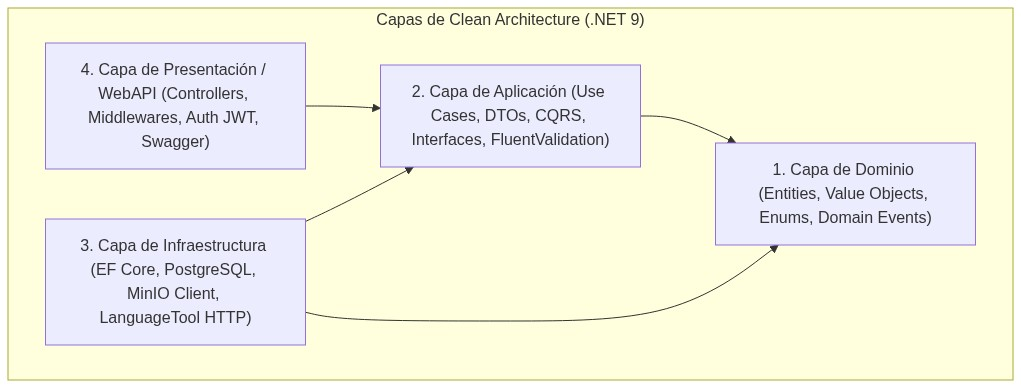
\includegraphics[width=0.80\textwidth,height=5.5cm,keepaspectratio]{images/s2_02_clean_architecture.png}
    \caption{Arquitectura Modular en Capas para Node.js + Express (v5).}
    \label{fig:s2_02_modular}
\end{figure}

\subsection{Diagrama de Contenedores C4 de la Solución}
El modelo C4 articula la interacción entre el cliente SPA y los servicios locales y externos:

\begin{figure}[htbp]
    \centering
    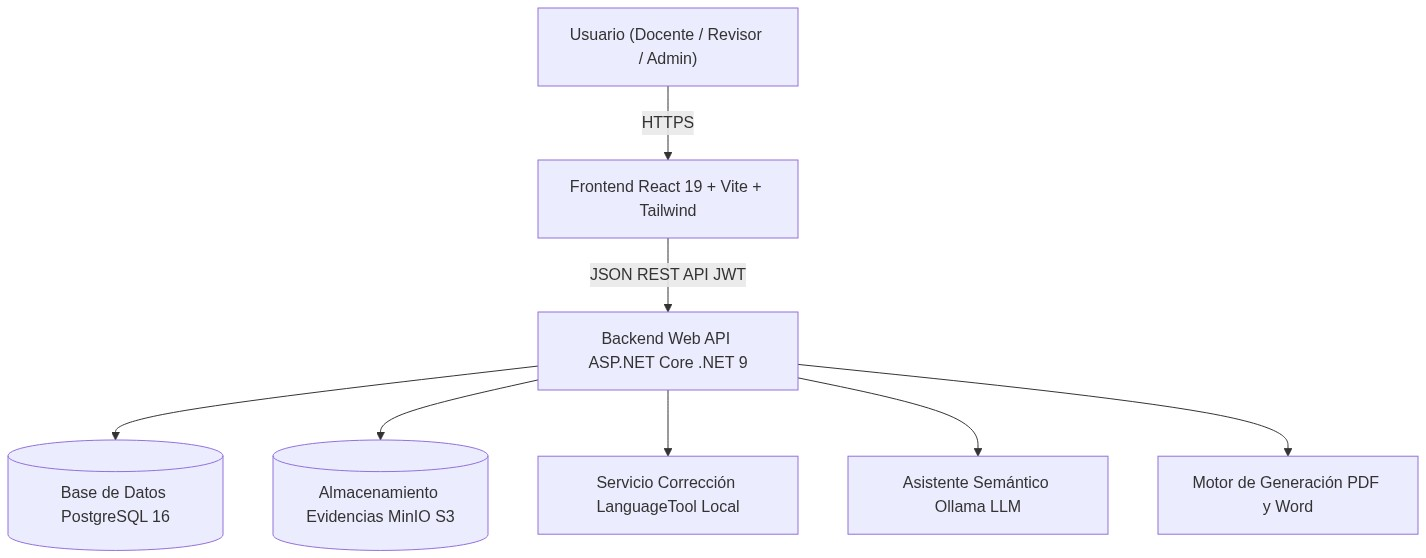
\includegraphics[width=0.82\textwidth,height=5.2cm,keepaspectratio]{images/s2_02_contenedores_c4.png}
    \caption{Diagrama de Contenedores del Modelo C4 para el Ecosistema SIGE.}
    \label{fig:s2_02_c4}
\end{figure}

\begin{itemize}[leftmargin=1.5em, itemsep=2pt]
    \item \textbf{Frontend SPA:} React + Vite con Tailwind CSS y CSS Keyframes institucionales (\texttt{\#00345E}).
    \item \textbf{Backend REST API:} Node.js + Express (v5) (puerto 5000) protegido por Helmet y Bearer JWT.
    \item \textbf{Base de Datos Relacional:} PostgreSQL 18 (puerto 5432) con almacenamiento ACID y pool de conexiones.
    \item \textbf{Almacenamiento de Evidencias:} MinIO S3 (puertos 9000 API y 9001 Consola Web).
    \item \textbf{Servicio de Corrección Sintáctica:} LanguageTool local en contenedor Docker (puerto 8010).
    \item \textbf{Asistente Semántico IA:} Inferencia delegada a Google Gemini API (Gemini 2.5 Flash / Google AI) mediante peticiones HTTPS seguras.
\end{itemize}

\section{Descripción de actividades}

\subsection{Estructura Monorepo Canónica del Proyecto (\texttt{SIGE/})}
\begin{lstlisting}
SIGE/
|-- .gitignore                  # Reglas de exclusion para Git (node_modules, .env, dist)
|-- package.json                # Configuracion raiz
|-- backend/
|   |-- src/
|   |   |-- config/             # Conexion PostgreSQL (pool) y entorno
|   |   |-- database/           # schema.sql, seed.sql y script init.js
|   |   |-- middlewares/        # auth.middleware, rateLimiter, errorHandler
|   |   |-- modules/
|   |   |   |-- auth/           # Controller, Service, Repository, Validation, Routes
|   |   |   `-- users/          # Controller, Service, Repository, Validation, Routes
|   |   |-- utils/              # password.util (bcrypt), token.util (JWT), response.util
|   |   |-- app.js              # Express app, CORS, Helmet, parseo JSON, rutas montadas
|   |   `-- server.js           # Inicio del servidor HTTP y escucha de conexiones
|   |-- .env                    # Variables locales (PORT, DB_*, JWT_SECRET)
|   |-- .env.example            # Plantilla de variables de entorno
|   `-- package.json            # Dependencias backend (express 5, pg, bcryptjs, jwt, helmet)
`-- frontend/
    |-- public/                 # Favicon y assets estaticos institucionales (logo-uta, logo-fisei)
    |-- src/
    |   |-- api/                # Cliente Axios con interceptor (JWT en header, auto-renovacion)
    |   |-- components/common/  # UI reutilizable: Button, Input, Modal, Card, Spinner
    |   |-- context/            # AuthContext (login, logout, estado del usuario)
    |   |-- pages/
    |   |   |-- LoginPage.jsx   # Pantalla de acceso institucional (#00345E, CSS Keyframes)
    |   |   `-- DashboardPage.jsx # Panel principal segun rol del usuario
    |   |-- App.jsx             # Rutas protegidas (react-router-dom)
    |   |-- main.jsx            # Punto de entrada React
    |   `-- index.css           # Directivas Tailwind, animaciones GPU y variables institucionales
    |-- .env                    # Variables del frontend (VITE_API_BASE_URL)
    |-- .env.example
    |-- tailwind.config.js      # Configuracion Tailwind (#00345E azul institucional UTA/FISEI)
    |-- vite.config.js          # Configuracion Vite y servidor de desarrollo
    `-- package.json            # Dependencias frontend (react, react-dom, axios, lucide-react)
\end{lstlisting}

\subsection{Patrones de Diseño Implementados}
\begin{enumerate}[leftmargin=1.5em, itemsep=2.5pt]
    \item \textbf{Modular Monolith \& Layered Architecture:} Cada dominio (\texttt{auth}, \texttt{users}, \texttt{reports}) agrupa sus rutas, validaciones, controladores, servicios y repositorios de forma desacoplada y mantenible.
    \item \textbf{Controller-Service-Repository:} Desacopla la gestión del protocolo HTTP (controlador) de las reglas de negocio (servicio) y el acceso a datos SQL puro parametrizado (repositorio).
    \item \textbf{Validation Gates en Middlewares:} Validación en cascada donde middlewares especializados rechazan peticiones con esquemas malformados o reglas de negocio incumplidas antes de ejecutar la lógica de aplicación.
    \item \textbf{Connection Pooling con \texttt{pg}:} Reutilización eficiente de conexiones abiertas hacia PostgreSQL 18 para maximizar el throughput y minimizar latencias en transacciones ACID.
    \item \textbf{Interceptor Pattern en Axios:} Interceptores de request para inyectar automáticamente el header \texttt{Authorization: Bearer <token>} e interceptores de response para gestionar la auto-renovación silenciosa con refresh token.
    \item \textbf{Defense in Depth con Helmet:} Aplicación de 11 middlewares de seguridad en Express v5 para mitigar ataques XSS, Clickjacking, MIME sniffing y degradación SSL.
\end{enumerate}

\subsection{Especificación de Seguridad y Token JWT}
\begin{itemize}[leftmargin=1.5em, itemsep=2pt]
    \item \textbf{Hashing de Contraseñas:} Bcrypt.js con factor de costo 12 para resistencia contra ataques de fuerza bruta.
    \item \textbf{Algoritmo de Firma Criptográfica:} HMAC-SHA256 con clave secreta de 512 bits inyectada por variable de entorno (\texttt{JWT\_SECRET}).
    \item \textbf{Tiempo de Expiración:} Access Token de 15 a 30 minutos y Refresh Token seguro con ciclo de vida de 7 días gestionado en la tabla \texttt{auth\_tokens} de PostgreSQL 18.
    \item \textbf{Claims Oficiales en el Token:}
    \begin{itemize}[leftmargin=1.2em, itemsep=1pt]
        \item \texttt{sub (UserId):} Identificador único universal del usuario (UUID).
        \item \texttt{email:} Correo electrónico institucional (\texttt{@uta.edu.ec}).
        \item \texttt{fullName:} Nombre completo del docente o directivo.
        \item \texttt{role:} Rol RBAC (\texttt{DocenteElaborador}, \texttt{CoordArea}, \texttt{CoordCarrera}, \texttt{Admin}).
        \item \texttt{facultadId} y \texttt{carreraId:} Pertenencia institucional a la FISEI e Ingeniería de Software.
    \end{itemize}
\end{itemize}

\vspace{0.3cm}

% =============================================================
% FIRMAS DE RESPONSABILIDAD
% =============================================================
\section{Firmas de Responsabilidad}

\noindent
\renewcommand{\arraystretch}{1.2}
\begin{tabularx}{\textwidth}{|>{\raggedright\arraybackslash}m{2.9cm}|>{\raggedright\arraybackslash}X|>{\centering\arraybackslash}m{4.6cm}|>{\centering\arraybackslash}m{2.3cm}|}
    \hline
    \rowcolor{headerred}
    \textcolor{white}{\textbf{ACCIÓN}} & \textcolor{white}{\textbf{NOMBRE Y CARGO}} & \textcolor{white}{\textbf{FIRMA}} & \textcolor{white}{\textbf{FECHA}} \\
    \hline
    \textbf{Elaborado por:} & Steeven Toala\newline \textit{Líder de Proyecto / Arquitecto Software} & \parbox[c]{4.4cm}{\centering\vspace{4pt}
\includegraphics[height=1.5cm,width=4.0cm,keepaspectratio]{images/firma_steveen.png}\vspace{4pt}} & 28/08/2026 \\
    \hline
    \textbf{Revisado por:} & Steeven Toala\newline \textit{Líder de Proyecto / Arquitecto Software} & \parbox[c]{4.4cm}{\centering\vspace{10pt}\textbf{\textcolor{gray!80}{\scriptsize [ PENDIENTE DE REVISIÓN ]}}\vspace{10pt}} & \textbf{\textcolor{gray!90}{Pendiente}} \\
    \hline
    \textbf{Aprobado por:} & Ing. Paulo Torres\newline \textit{Docente Tutor - Gestión Proyectos Software} & \parbox[c]{4.4cm}{\centering\vspace{10pt}\textbf{\textcolor{gray!80}{\scriptsize [ PENDIENTE DE APROBACIÓN ]}}\vspace{10pt}} & \textbf{\textcolor{gray!90}{Pendiente}} \\
    \hline
\end{tabularx}

\vspace{0.4cm}

% =============================================================
% CONTROL DE CAMBIOS
% =============================================================
\section{Control de Cambios}

\noindent
\renewcommand{\arraystretch}{1.2}
\begin{tabularx}{\textwidth}{|>{\hsize=0.45\hsize\centering\arraybackslash}X|>{\hsize=1.55\hsize\raggedright\arraybackslash}X|>{\hsize=1.2\hsize\raggedright\arraybackslash}X|>{\hsize=0.8\hsize\centering\arraybackslash}X|}
    \hline
    \rowcolor{gray!20}
    \textbf{Versión} & \textbf{Descripción del cambio} & \textbf{Responsable del cambio} & \textbf{Fecha de aprobación} \\
    \hline
    1.0 & Diseño de arquitectura modular en capas Node.js + Express (v5), PostgreSQL 18, React + Vite, modelo C4 y especificacion JWT/Helmet & Steeven Toala & \textbf{\textcolor{gray!90}{Pendiente de Revisión}} \\
    \hline
\end{tabularx}

\vspace{0.4cm}

\section{Anexos}
\subsection*{Anexo 1: Inicialización del Servidor HTTP y Middlewares en Express (v5)}
Configuración centralizada en \texttt{app.js} y \texttt{server.js} que demuestra el montaje de Helmet, CORS, parseo JSON, pool de PostgreSQL 18 y el enrutador modular para autenticación y usuarios.

\end{document}
